% Options for packages loaded elsewhere
\PassOptionsToPackage{unicode}{hyperref}
\PassOptionsToPackage{hyphens}{url}
%
\documentclass[
  ignorenonframetext,
]{beamer}
\usepackage{pgfpages}
\setbeamertemplate{caption}[numbered]
\setbeamertemplate{caption label separator}{: }
\setbeamercolor{caption name}{fg=normal text.fg}
\beamertemplatenavigationsymbolsempty
% Prevent slide breaks in the middle of a paragraph
\widowpenalties 1 10000
\raggedbottom
\setbeamertemplate{part page}{
  \centering
  \begin{beamercolorbox}[sep=16pt,center]{part title}
    \usebeamerfont{part title}\insertpart\par
  \end{beamercolorbox}
}
\setbeamertemplate{section page}{
  \centering
  \begin{beamercolorbox}[sep=12pt,center]{part title}
    \usebeamerfont{section title}\insertsection\par
  \end{beamercolorbox}
}
\setbeamertemplate{subsection page}{
  \centering
  \begin{beamercolorbox}[sep=8pt,center]{part title}
    \usebeamerfont{subsection title}\insertsubsection\par
  \end{beamercolorbox}
}
\AtBeginPart{
  \frame{\partpage}
}
\AtBeginSection{
  \ifbibliography
  \else
    \frame{\sectionpage}
  \fi
}
\AtBeginSubsection{
  \frame{\subsectionpage}
}
\usepackage{lmodern}
\usepackage{amssymb,amsmath}
\usepackage{ifxetex,ifluatex}
\ifnum 0\ifxetex 1\fi\ifluatex 1\fi=0 % if pdftex
  \usepackage[T1]{fontenc}
  \usepackage[utf8]{inputenc}
  \usepackage{textcomp} % provide euro and other symbols
\else % if luatex or xetex
  \usepackage{unicode-math}
  \defaultfontfeatures{Scale=MatchLowercase}
  \defaultfontfeatures[\rmfamily]{Ligatures=TeX,Scale=1}
\fi
\usetheme[]{Hannover}
\usecolortheme{dove}
\usefonttheme{structurebold}
% Use upquote if available, for straight quotes in verbatim environments
\IfFileExists{upquote.sty}{\usepackage{upquote}}{}
\IfFileExists{microtype.sty}{% use microtype if available
  \usepackage[]{microtype}
  \UseMicrotypeSet[protrusion]{basicmath} % disable protrusion for tt fonts
}{}
\makeatletter
\@ifundefined{KOMAClassName}{% if non-KOMA class
  \IfFileExists{parskip.sty}{%
    \usepackage{parskip}
  }{% else
    \setlength{\parindent}{0pt}
    \setlength{\parskip}{6pt plus 2pt minus 1pt}}
}{% if KOMA class
  \KOMAoptions{parskip=half}}
\makeatother
\usepackage{xcolor}
\IfFileExists{xurl.sty}{\usepackage{xurl}}{} % add URL line breaks if available
\IfFileExists{bookmark.sty}{\usepackage{bookmark}}{\usepackage{hyperref}}
\hypersetup{
  pdftitle={Session 2: Linear and logistic regression as Generalized Linear Models},
  pdfauthor={Levi Waldron},
  hidelinks,
  pdfcreator={LaTeX via pandoc}}
\urlstyle{same} % disable monospaced font for URLs
\newif\ifbibliography
\usepackage{color}
\usepackage{fancyvrb}
\newcommand{\VerbBar}{|}
\newcommand{\VERB}{\Verb[commandchars=\\\{\}]}
\DefineVerbatimEnvironment{Highlighting}{Verbatim}{commandchars=\\\{\}}
% Add ',fontsize=\small' for more characters per line
\usepackage{framed}
\definecolor{shadecolor}{RGB}{248,248,248}
\newenvironment{Shaded}{\begin{snugshade}}{\end{snugshade}}
\newcommand{\AlertTok}[1]{\textcolor[rgb]{0.94,0.16,0.16}{#1}}
\newcommand{\AnnotationTok}[1]{\textcolor[rgb]{0.56,0.35,0.01}{\textbf{\textit{#1}}}}
\newcommand{\AttributeTok}[1]{\textcolor[rgb]{0.77,0.63,0.00}{#1}}
\newcommand{\BaseNTok}[1]{\textcolor[rgb]{0.00,0.00,0.81}{#1}}
\newcommand{\BuiltInTok}[1]{#1}
\newcommand{\CharTok}[1]{\textcolor[rgb]{0.31,0.60,0.02}{#1}}
\newcommand{\CommentTok}[1]{\textcolor[rgb]{0.56,0.35,0.01}{\textit{#1}}}
\newcommand{\CommentVarTok}[1]{\textcolor[rgb]{0.56,0.35,0.01}{\textbf{\textit{#1}}}}
\newcommand{\ConstantTok}[1]{\textcolor[rgb]{0.00,0.00,0.00}{#1}}
\newcommand{\ControlFlowTok}[1]{\textcolor[rgb]{0.13,0.29,0.53}{\textbf{#1}}}
\newcommand{\DataTypeTok}[1]{\textcolor[rgb]{0.13,0.29,0.53}{#1}}
\newcommand{\DecValTok}[1]{\textcolor[rgb]{0.00,0.00,0.81}{#1}}
\newcommand{\DocumentationTok}[1]{\textcolor[rgb]{0.56,0.35,0.01}{\textbf{\textit{#1}}}}
\newcommand{\ErrorTok}[1]{\textcolor[rgb]{0.64,0.00,0.00}{\textbf{#1}}}
\newcommand{\ExtensionTok}[1]{#1}
\newcommand{\FloatTok}[1]{\textcolor[rgb]{0.00,0.00,0.81}{#1}}
\newcommand{\FunctionTok}[1]{\textcolor[rgb]{0.00,0.00,0.00}{#1}}
\newcommand{\ImportTok}[1]{#1}
\newcommand{\InformationTok}[1]{\textcolor[rgb]{0.56,0.35,0.01}{\textbf{\textit{#1}}}}
\newcommand{\KeywordTok}[1]{\textcolor[rgb]{0.13,0.29,0.53}{\textbf{#1}}}
\newcommand{\NormalTok}[1]{#1}
\newcommand{\OperatorTok}[1]{\textcolor[rgb]{0.81,0.36,0.00}{\textbf{#1}}}
\newcommand{\OtherTok}[1]{\textcolor[rgb]{0.56,0.35,0.01}{#1}}
\newcommand{\PreprocessorTok}[1]{\textcolor[rgb]{0.56,0.35,0.01}{\textit{#1}}}
\newcommand{\RegionMarkerTok}[1]{#1}
\newcommand{\SpecialCharTok}[1]{\textcolor[rgb]{0.00,0.00,0.00}{#1}}
\newcommand{\SpecialStringTok}[1]{\textcolor[rgb]{0.31,0.60,0.02}{#1}}
\newcommand{\StringTok}[1]{\textcolor[rgb]{0.31,0.60,0.02}{#1}}
\newcommand{\VariableTok}[1]{\textcolor[rgb]{0.00,0.00,0.00}{#1}}
\newcommand{\VerbatimStringTok}[1]{\textcolor[rgb]{0.31,0.60,0.02}{#1}}
\newcommand{\WarningTok}[1]{\textcolor[rgb]{0.56,0.35,0.01}{\textbf{\textit{#1}}}}
\usepackage{graphicx,grffile}
\makeatletter
\def\maxwidth{\ifdim\Gin@nat@width>\linewidth\linewidth\else\Gin@nat@width\fi}
\def\maxheight{\ifdim\Gin@nat@height>\textheight\textheight\else\Gin@nat@height\fi}
\makeatother
% Scale images if necessary, so that they will not overflow the page
% margins by default, and it is still possible to overwrite the defaults
% using explicit options in \includegraphics[width, height, ...]{}
\setkeys{Gin}{width=\maxwidth,height=\maxheight,keepaspectratio}
% Set default figure placement to htbp
\makeatletter
\def\fps@figure{htbp}
\makeatother
\setlength{\emergencystretch}{3em} % prevent overfull lines
\providecommand{\tightlist}{%
  \setlength{\itemsep}{0pt}\setlength{\parskip}{0pt}}
\setcounter{secnumdepth}{-\maxdimen} % remove section numbering

\title{Session 2: Linear and logistic regression as Generalized Linear Models}
\author{Levi Waldron}
\date{}
\institute{CUNY SPH Biostatistics 2}

\begin{document}
\frame{\titlepage}

\hypertarget{learning-objectives-and-outline}{%
\section{Learning Objectives and
Outline}\label{learning-objectives-and-outline}}

\begin{frame}{Learning objectives}
\protect\hypertarget{learning-objectives}{}

\begin{enumerate}
\tightlist
\item
  define generalized linear models (GLM)
\item
  define linear and logistic regression as special cases of GLMs
\item
  distinguish between additive and multiplicative models
\item
  define Pearson and deviance residuals
\item
  describe application of the Wald test
\end{enumerate}

\end{frame}

\begin{frame}{Outline}
\protect\hypertarget{outline}{}

\begin{enumerate}
\tightlist
\item
  Brief overview of multiple regression (Vittinghoff 4.1-4.3)
\item
  Linear Regression as a GLM (Vittinghoff 4.1-4.3)
\item
  Logistic Regression as a GLM (Vittinghoff 5.1-5.3)
\item
  Statistical inference for logistic regression (Vittinghoff 5.1-5.3)
\end{enumerate}

\end{frame}

\hypertarget{review-of-multiple-linear-regression}{%
\section{Review of multiple linear
regression}\label{review-of-multiple-linear-regression}}

\begin{frame}{Systematic component}
\protect\hypertarget{systematic-component}{}

\[
E[y|x] = \beta_0 + \beta_1 x_1 + \beta_2 x_2 + ... + \beta_p x_p
\]

\begin{itemize}
\tightlist
\item
  \(x_p\) are the predictors or independent variables
\item
  \(y\) is the outcome, response, or dependent variable
\item
  \(E[y|x]\) is the expected value of \(y\) given \(x\)
\item
  \(\beta_p\) are the regression coefficients
\end{itemize}

\end{frame}

\begin{frame}{Systematic plus random component}
\protect\hypertarget{systematic-plus-random-component}{}

\(y_i = E[y|x] + \epsilon_i\)

\(y_i = \beta_0 + \beta_1 x_1 + \beta_2 x_2 + ... + \beta_p x_p + \epsilon_i\)

Assumption: \(\epsilon_i \stackrel{iid}{\sim} N(0, \sigma_\epsilon^2)\)

\begin{itemize}
\tightlist
\item
  Normal distribution
\item
  Mean zero at every value of predictors
\item
  Constant variance at every value of predictors
\item
  Values that are statistically independent
\end{itemize}

\end{frame}

\hypertarget{linear-regression-as-a-glm}{%
\section{Linear Regression as a GLM}\label{linear-regression-as-a-glm}}

\begin{frame}{Generalized Linear Models (GLM)}
\protect\hypertarget{generalized-linear-models-glm}{}

\begin{itemize}
\tightlist
\item
  Linear regression is a special case of a broad family of models called
  ``Generalized Linear Models'' (GLM)
\item
  This unifying approach allows to fit a large set of models using
  maximum likelihood estimation methods (MLE) (Nelder \& Wedderburn,
  1972)
\item
  Can model many types of data directly using appropriate distributions,
  e.g.~Poisson distribution for count data
\item
  Transformations of \(Y\) not needed
\end{itemize}

\end{frame}

\begin{frame}{Components of GLM}
\protect\hypertarget{components-of-glm}{}

\begin{itemize}
\tightlist
\item
  \textbf{Random component} specifies the conditional distribution for
  the response variable

  \begin{itemize}
  \tightlist
  \item
    doesn't have to be normal
  \item
    can be any distribution in the ``exponential'' family of
    distributions
  \end{itemize}
\item
  \textbf{Systematic component} specifies linear function of predictors
  (linear predictor)
\item
  \textbf{Link} {[}denoted by g(.){]} specifies the relationship between
  the expected value of the random component and the systematic
  component

  \begin{itemize}
  \tightlist
  \item
    can be linear or nonlinear
  \end{itemize}
\end{itemize}

\end{frame}

\begin{frame}{Linear Regression as GLM}
\protect\hypertarget{linear-regression-as-glm}{}

\begin{itemize}
\item
  \textbf{The model}:
  \(y_i = E[y|x] + \epsilon_i = \beta_0 + \beta_1 x_{1i} + \beta_2 x_{2i} + ... + \beta_p x_{pi} + \epsilon_i\)
\item
  \textbf{Random component} of \(y_i\) is normally distributed:
  \(\epsilon_i \stackrel{iid}{\sim} N(0, \sigma_\epsilon^2)\)
\item
  \textbf{Systematic component} (linear predictor):
  \(\beta_0 + \beta_1 x_{1i} + \beta_2 x_{2i} + ... + \beta_p x_{pi}\)
\item
  \textbf{Link function} here is the \emph{identity link}:
  \(g(E(y | x)) = E(y | x)\). We are modeling the mean directly, no
  transformation.
\end{itemize}

\end{frame}

\hypertarget{logistic-regression-as-a-glm}{%
\section{Logistic Regression as a
GLM}\label{logistic-regression-as-a-glm}}

\begin{frame}{The logistic regression model}
\protect\hypertarget{the-logistic-regression-model}{}

\begin{itemize}
\item
  \textbf{The model}: \[
  Logit(P(x)) = log \left( \frac{P(x)}{1-P(x)} \right) = \beta_0 + \beta_1 x_{1i} + \beta_2 x_{2i} + ... + \beta_p x_{pi}
  \]
\item
  \textbf{Random component}: \(y_i\) follows a Binomial distribution
  (outcome is a binary variable)
\item
  \textbf{Systematic component}: linear predictor \[
  \beta_0 + \beta_1 x_{1i} + \beta_2 x_{2i} + ... + \beta_p x_{pi}
  \]
\item
  \textbf{Link function}: \emph{logit} (log of the odds that the event
  occurs)
\end{itemize}

\[
g(P(x)) = logit(P(x)) = log\left( \frac{P(x)}{1-P(x)} \right)
\]

\[
P(x) = g^{-1}\left( \beta_0 + \beta_1 x_{1i} + \beta_2 x_{2i} + ... + \beta_p x_{pi}
 \right)
\]

\end{frame}

\begin{frame}[fragile]{The logit function}
\protect\hypertarget{the-logit-function}{}

\small

\begin{Shaded}
\begin{Highlighting}[]
\NormalTok{logit <-}\StringTok{ }\ControlFlowTok{function}\NormalTok{(P) }\KeywordTok{log}\NormalTok{(P}\OperatorTok{/}\NormalTok{(}\DecValTok{1}\OperatorTok{-}\NormalTok{P))}
\KeywordTok{plot}\NormalTok{(logit, }\DataTypeTok{xlab=}\StringTok{"Probability"}\NormalTok{, }\DataTypeTok{ylab=}\StringTok{"Log-odds"}\NormalTok{,}
     \DataTypeTok{cex.lab=}\FloatTok{1.5}\NormalTok{, }\DataTypeTok{cex.axis=}\FloatTok{1.5}\NormalTok{)}
\end{Highlighting}
\end{Shaded}

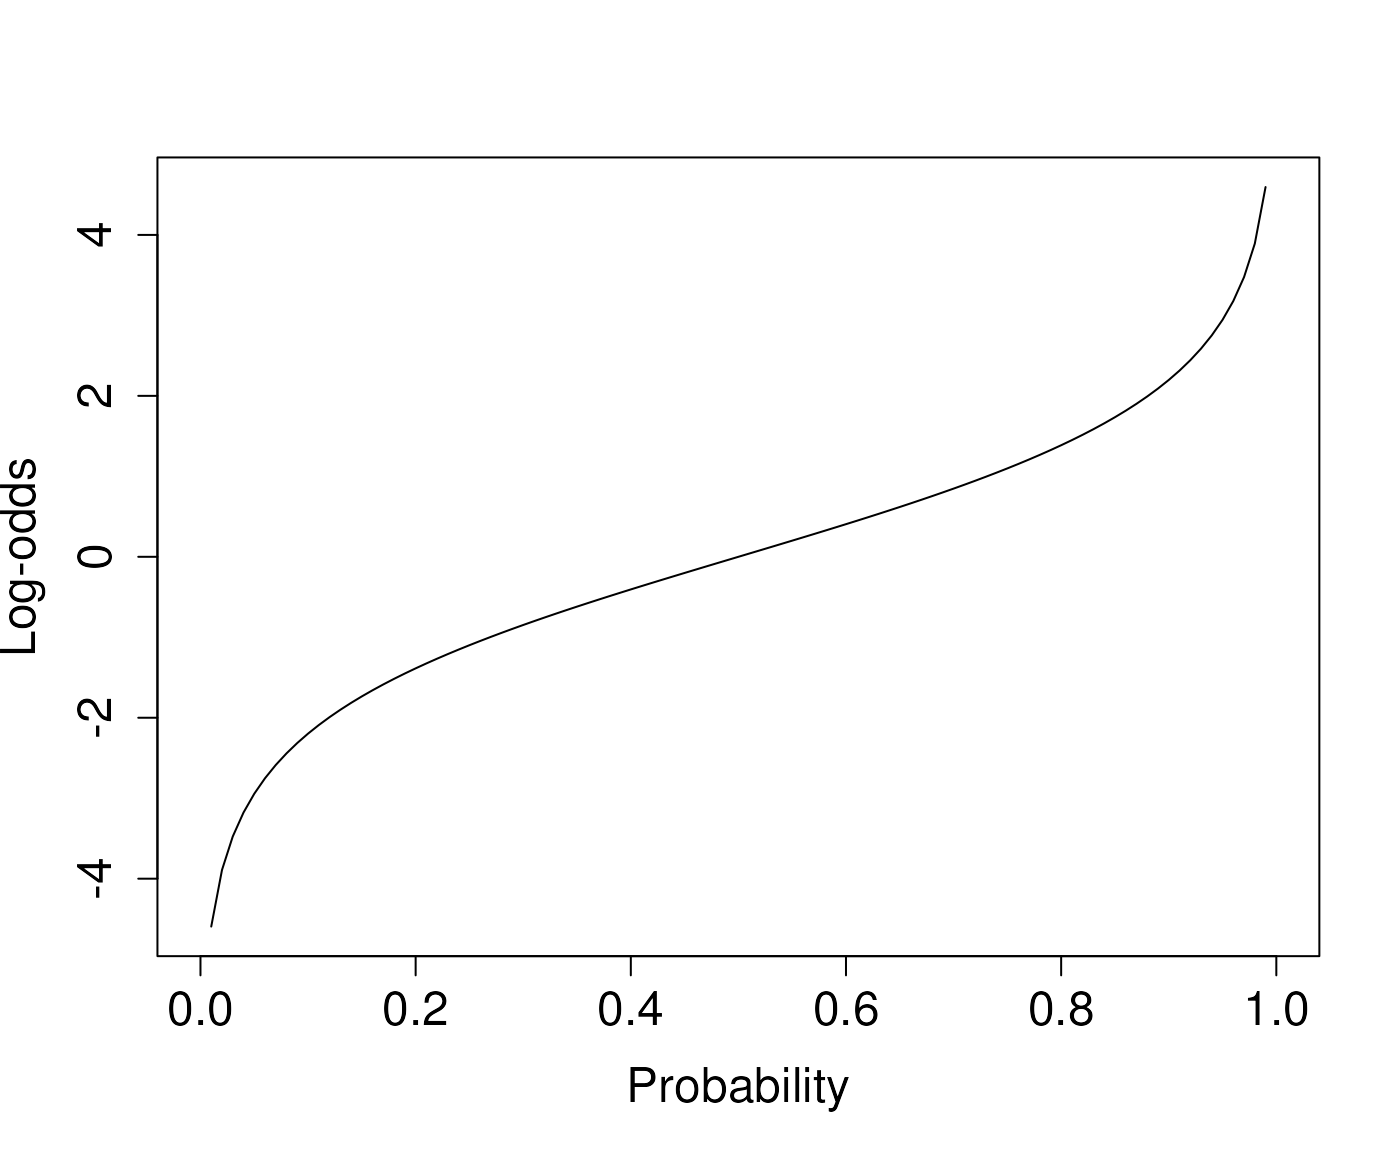
\includegraphics{../docs/articles/session_lecture_files/figure-beamer/unnamed-chunk-1-1.pdf}

\end{frame}

\begin{frame}[fragile]{Inverse logit function}
\protect\hypertarget{inverse-logit-function}{}

\begin{Shaded}
\begin{Highlighting}[]
\NormalTok{invLogit <-}\StringTok{ }\ControlFlowTok{function}\NormalTok{(x) }\DecValTok{1}\OperatorTok{/}\NormalTok{(}\DecValTok{1}\OperatorTok{+}\KeywordTok{exp}\NormalTok{(}\OperatorTok{-}\NormalTok{x))}
\end{Highlighting}
\end{Shaded}

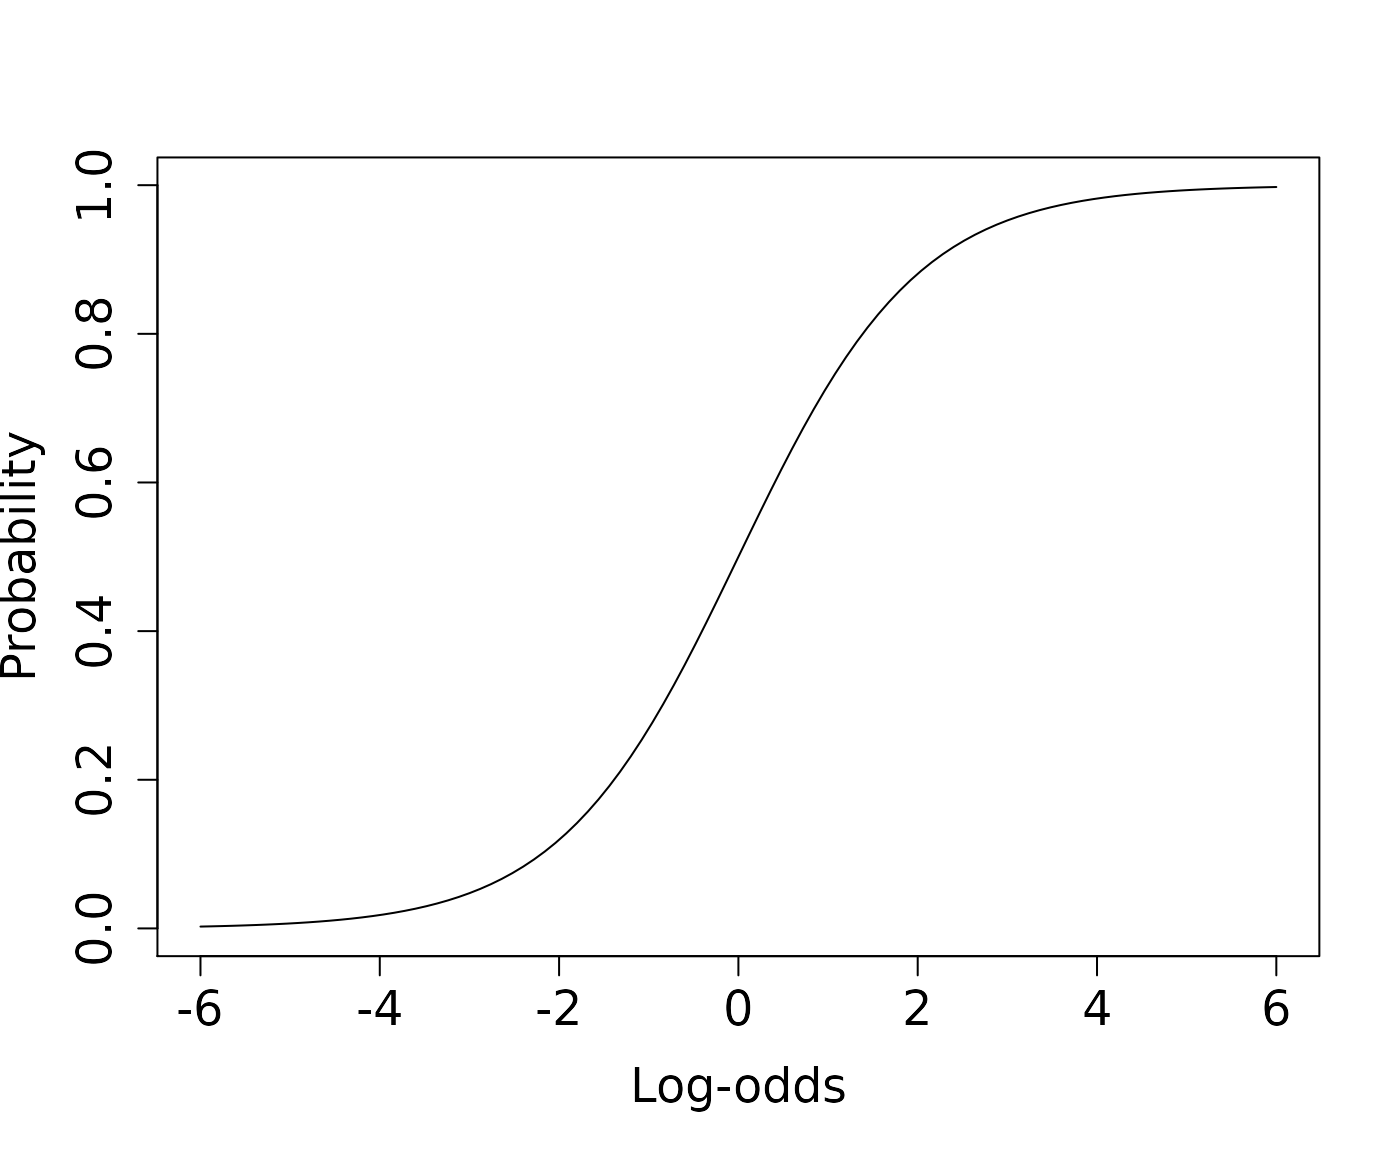
\includegraphics{../docs/articles/session_lecture_files/figure-beamer/unnamed-chunk-3-1.pdf}

\end{frame}

\begin{frame}[fragile]{Example: contraceptive use data}
\protect\hypertarget{example-contraceptive-use-data}{}

Load the contraceptive use data

\tiny

\begin{Shaded}
\begin{Highlighting}[]
\KeywordTok{suppressPackageStartupMessages}\NormalTok{(}\KeywordTok{library}\NormalTok{(dplyr))}
\NormalTok{cuse <-}\StringTok{ }\KeywordTok{read.table}\NormalTok{(}\StringTok{"cuse.dat"}\NormalTok{, }\DataTypeTok{header=}\OtherTok{TRUE}\NormalTok{)}
\NormalTok{cuse <-}\StringTok{ }\KeywordTok{mutate}\NormalTok{(cuse, }\DataTypeTok{percentusing =}\NormalTok{ using }\OperatorTok{/}\StringTok{ }\NormalTok{(using }\OperatorTok{+}\StringTok{ }\NormalTok{notUsing) }\OperatorTok{*}\StringTok{ }\DecValTok{100}\NormalTok{) }\OperatorTok
\StringTok{  }\KeywordTok{mutate}\NormalTok{(}\DataTypeTok{n =}\NormalTok{ using }\OperatorTok{+}\StringTok{ }\NormalTok{notUsing)}
\NormalTok{cuse}
\end{Highlighting}
\end{Shaded}

Source: \url{http://data.princeton.edu/wws509/datasets/\#cuse}

\end{frame}

\begin{frame}[fragile]{Table One}
\protect\hypertarget{table-one}{}

\tiny

\begin{verbatim}
##                           Stratified by age
##                            Overall       <25           25-29        
##   n                           16             4             4        
##   education = low (%)          8 (50.0)      2 (50.0)      2 (50.0) 
##   wantsMore = yes (%)          8 (50.0)      2 (50.0)      2 (50.0) 
##   percentusing (mean (SD)) 32.92 (17.51) 18.78 (7.64)  27.15 (6.53) 
##                           Stratified by age
##                            30-39         40-49        
##   n                            4             4        
##   education = low (%)          2 (50.0)      2 (50.0) 
##   wantsMore = yes (%)          2 (50.0)      2 (50.0) 
##   percentusing (mean (SD)) 38.80 (15.65) 46.95 (23.82)
\end{verbatim}

\footnotesize

See
\href{https://cran.r-project.org/web/packages/tableone/vignettes/introduction.html}{tableone}
vignette for e.g.~how to export to Word / Excel

\url{https://cran.r-project.org/web/packages/tableone/vignettes/introduction.html}

\end{frame}

\begin{frame}[fragile]{Perform regression}
\protect\hypertarget{perform-regression}{}

\tiny

\begin{Shaded}
\begin{Highlighting}[]
\NormalTok{fit1 <-}\StringTok{ }\KeywordTok{glm}\NormalTok{(}\KeywordTok{cbind}\NormalTok{(using, notUsing) }\OperatorTok{~}\StringTok{ }\NormalTok{age }\OperatorTok{+}\StringTok{ }\NormalTok{education }\OperatorTok{+}\StringTok{ }\NormalTok{wantsMore, }
           \DataTypeTok{data=}\NormalTok{cuse, }\DataTypeTok{family=}\KeywordTok{binomial}\NormalTok{(}\StringTok{"logit"}\NormalTok{))}
\KeywordTok{summary}\NormalTok{(fit1)}
\end{Highlighting}
\end{Shaded}

\begin{verbatim}
## 
## Call:
## glm(formula = cbind(using, notUsing) ~ age + education + wantsMore, 
##     family = binomial("logit"), data = cuse)
## 
## Deviance Residuals: 
##     Min       1Q   Median       3Q      Max  
## -2.5148  -0.9376   0.2408   0.9822   1.7333  
## 
## Coefficients:
##              Estimate Std. Error z value Pr(>|z|)    
## (Intercept)   -0.8082     0.1590  -5.083 3.71e-07 ***
## age25-29       0.3894     0.1759   2.214  0.02681 *  
## age30-39       0.9086     0.1646   5.519 3.40e-08 ***
## age40-49       1.1892     0.2144   5.546 2.92e-08 ***
## educationlow  -0.3250     0.1240  -2.620  0.00879 ** 
## wantsMoreyes  -0.8330     0.1175  -7.091 1.33e-12 ***
## ---
## Signif. codes:  0 '***' 0.001 '**' 0.01 '*' 0.05 '.' 0.1 ' ' 1
## 
## (Dispersion parameter for binomial family taken to be 1)
## 
##     Null deviance: 165.772  on 15  degrees of freedom
## Residual deviance:  29.917  on 10  degrees of freedom
## AIC: 113.43
## 
## Number of Fisher Scoring iterations: 4
\end{verbatim}

\end{frame}

\hypertarget{residuals-for-logistic-regression}{%
\section{Residuals for logistic
regression}\label{residuals-for-logistic-regression}}

\begin{frame}{Pearson residuals for logistic regression}
\protect\hypertarget{pearson-residuals-for-logistic-regression}{}

\begin{itemize}
\tightlist
\item
  Traditional residuals \(y_i - E[y_i|x_i]\) don't make sense for binary
  \(y\).
\item
  One alternative is \emph{Pearson residuals}

  \begin{itemize}
  \tightlist
  \item
    take the difference between observed and fitted values (on
    probability scale 0-1), and divide by the standard deviation of the
    observed value.
  \end{itemize}
\item
  Let \(\hat y_i\) be the best-fit predicted probability for each data
  point, i.e.~\(g^{-1}(\beta_0 + \beta_1 x_{1i} + ...)\)
\item
  \(y_i\) is the observed value, either 0 or 1.
\end{itemize}

\[
r_i = \frac{y_i - \hat y_i}{ \sqrt{ Var(\hat y_i) }}
\]

Summing the squared Pearson residuals produces the \emph{Pearson
Chi-squared statistic}:

\[
\chi ^2 = \sum_i r_i^2
\]

\end{frame}

\begin{frame}{Deviance residuals for logistic regression}
\protect\hypertarget{deviance-residuals-for-logistic-regression}{}

\begin{itemize}
\tightlist
\item
  Deviance residuals and Pearson residuals converge for high degrees of
  freedom
\item
  Deviance residuals indicate the contribution of each point to the
  model \emph{likelihood}
\item
  Definition of deviance residuals:
\end{itemize}

\[
d_i = s_i \sqrt{ -2 ( y_i \log \hat y_i + (1-y_i) \log (1 - \hat y_i) ) }
\]

Where \(s_i = 1\) if \(y_i = 1\) and \(s_i = -1\) if \(y_i = 0\).

\begin{itemize}
\tightlist
\item
  Summing the deviances gives the overall deviance: \(D = \sum_i d_i^2\)
\end{itemize}

\end{frame}

\hypertarget{likelihood-and-hypothesis-testing}{%
\section{Likelihood and hypothesis
testing}\label{likelihood-and-hypothesis-testing}}

\begin{frame}{What is likelihood?}
\protect\hypertarget{what-is-likelihood}{}

\begin{itemize}
\tightlist
\item
  The \emph{likelihood} of a model is the probability of the observed
  outcomes given the model, sometimes written as:

  \begin{itemize}
  \tightlist
  \item
    \(L(\theta | data) = P(data|\theta)\).
  \end{itemize}
\item
  Deviance residuals and the difference in log-likelihood between two
  models are related by:
\end{itemize}

\(\Delta (\textrm{D}) = -2 * \Delta (\textrm{log likelihood})\)

\end{frame}

\begin{frame}{Likelihood Ratio Test}
\protect\hypertarget{likelihood-ratio-test}{}

\begin{itemize}
\tightlist
\item
  Use to assess whether the reduction in deviance provided by a more
  complicated model indicates a better fit
\item
  It is equivalent of the nested Analysis of Variance is a nested
  Analysis of Deviance
\item
  The difference in deviance under \(H_0\) is \emph{chi-square
  distributed}, with df equal to the difference in df of the two models.
\end{itemize}

\end{frame}

\begin{frame}[fragile]{Likelihood Ratio Test (cont'd)}
\protect\hypertarget{likelihood-ratio-test-contd}{}

\scriptsize

\begin{Shaded}
\begin{Highlighting}[]
\NormalTok{fit0 <-}\StringTok{ }\KeywordTok{glm}\NormalTok{(}\KeywordTok{cbind}\NormalTok{(using, notUsing) }\OperatorTok{~}\StringTok{ }\DecValTok{-1}\NormalTok{, }\DataTypeTok{data=}\NormalTok{cuse, }
            \DataTypeTok{family=}\KeywordTok{binomial}\NormalTok{(}\StringTok{"logit"}\NormalTok{))}
\KeywordTok{anova}\NormalTok{(fit0, fit1, }\DataTypeTok{test=}\StringTok{"LRT"}\NormalTok{)}
\end{Highlighting}
\end{Shaded}

\end{frame}

\begin{frame}{Wald test for individual regression coefficients}
\protect\hypertarget{wald-test-for-individual-regression-coefficients}{}

\begin{itemize}
\tightlist
\item
  Can use partial Wald test for a single coefficient:

  \begin{itemize}
  \tightlist
  \item
    \(\frac{\hat{\beta}}{\sqrt{var(\hat{\beta)}}} \sim t_{n-1}\)
  \item
    \(\frac{\left ( \hat{\beta} - \beta_0 \right )^2 }{var(\hat{\beta)}} \sim \chi^2_{df=1}\)
    (large sample)
  \end{itemize}
\item
  Wald CI for \(\beta\):
  \(\hat{\beta} \pm t_{1-\alpha/2, n-1} \sqrt{var(\hat{\beta})}\)
\item
  Wald CI for odds-ratio:
  \(e^{\hat{\beta} \pm t_{1-\alpha/2, n-1} \sqrt{var(\hat{\beta})}}\)
\end{itemize}

\emph{Note}: Wald test confidence intervals on coefficients can provide
poor coverage in some cases, even with relatively large samples

\end{frame}

\hypertarget{additive-vs.-multiplicative-models}{%
\section{Additive vs.~Multiplicative
models}\label{additive-vs.-multiplicative-models}}

\begin{frame}{Additive vs.~Multiplicative models}
\protect\hypertarget{additive-vs.-multiplicative-models-1}{}

\begin{itemize}
\tightlist
\item
  Linear regression is an \emph{additive} model

  \begin{itemize}
  \tightlist
  \item
    \emph{e.g.} for two binary variables \(\beta_1 = 1.5\),
    \(\beta_2 = 1.5\).
  \item
    If \(x_1=1\) and \(x_2=1\), this adds 3.0 to \(E(y|x)\)
  \end{itemize}
\item
  Logistic regression is a \emph{multiplicative} model

  \begin{itemize}
  \tightlist
  \item
    If \(x_1=1\) and \(x_2=1\), this adds 3.0 to \(log(\frac{P}{1-P})\)
  \item
    Odds-ratio \(\frac{P}{1-P}\) increases 20-fold: \(exp(1.5+1.5)\) or
    \(exp(1.5) * exp(1.5)\)
  \end{itemize}
\end{itemize}

\end{frame}

\end{document}
